\documentclass[border=2pt]{standalone}
\usepackage{tikz}\usetikzlibrary{arrows.meta,positioning,shapes.geometric,calc}
\usepackage[T1]{fontenc}\usepackage{lmodern}
\begin{document}
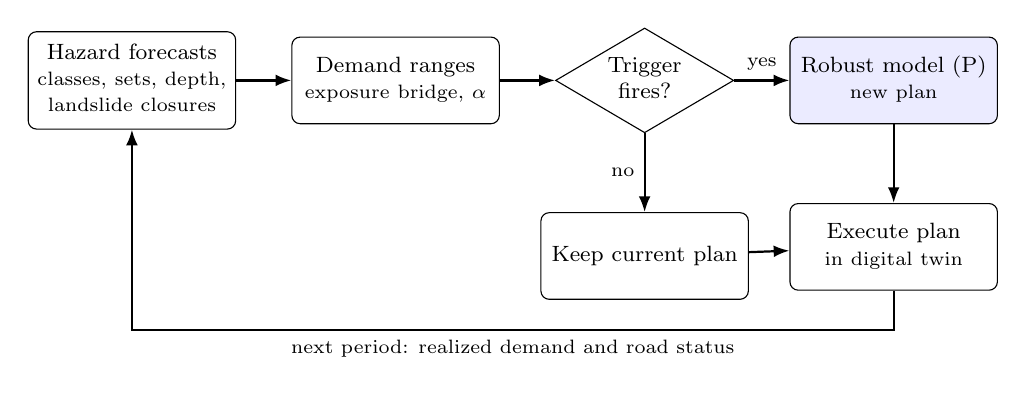
\begin{tikzpicture}[
  node distance=6mm and 7mm,
  box/.style={draw, rounded corners=3pt, align=center, minimum height=11mm, text width=24mm, font=\footnotesize},
  dec/.style={draw, diamond, aspect=1.7, align=center, inner sep=1pt, font=\footnotesize},
  arr/.style={-{Latex[length=2mm]}, thick}]
\node[box] (fc) {\begin{tabular}{@{}c@{}}\footnotesize Hazard forecasts\\\fontsize{7pt}{8pt}\selectfont classes, sets, depth,\\\fontsize{7pt}{8pt}\selectfont landslide closures\end{tabular}};
\node[box, right=of fc] (us) {\begin{tabular}{@{}c@{}}\footnotesize Demand ranges\\\fontsize{7pt}{8pt}\selectfont exposure bridge, $\alpha$\end{tabular}};
\node[dec, right=of us] (tr) {\begin{tabular}{@{}c@{}}\footnotesize Trigger\\\footnotesize fires?\end{tabular}};
\node[box, right=of tr, fill=blue!8] (rm) {\begin{tabular}{@{}c@{}}\footnotesize Robust model (P)\\\fontsize{7pt}{8pt}\selectfont new plan\end{tabular}};
\node[box, below=10mm of tr] (kp) {\footnotesize Keep current plan};
\node[box, below=10mm of rm] (ex) {\begin{tabular}{@{}c@{}}\footnotesize Execute plan\\\fontsize{7pt}{8pt}\selectfont in digital twin\end{tabular}};
\draw[arr] (fc) -- (us);
\draw[arr] (us) -- (tr);
\draw[arr] (tr) -- node[above, font=\fontsize{7pt}{8pt}\selectfont]{yes} (rm);
\draw[arr] (tr) -- node[left, font=\fontsize{7pt}{8pt}\selectfont]{no} (kp);
\draw[arr] (rm) -- (ex);
\draw[arr] (kp) -- (ex);
\draw[arr] (ex.south) -- ++(0,-5mm) -| node[pos=0.25, below, font=\fontsize{7pt}{8pt}\selectfont]{next period: realized demand and road status} (fc.south);
\end{tikzpicture}
\end{document}
